\section{Related Work}
\label{sec:related-work}
 
We review prior work on quantization, low-voltage induced random bit errors and weight robustness; \revision{more in \appref{sec:supp-related-work}.}
 
\textbf{Quantization:} DNN Quantization \citep{GuoARXIV2018b} is usually motivated by faster 
DNN inference, \eg, through fixed-point quantization and arithmetic \citep{ShinICASSP2017,LinICML2016,LiNIPS2017}, and energy savings. To avoid reduced accuracy, quantization is considered during training \citep{JacobCVPR2018,KrishnamoorthiARXIV2018} instead of post-training or with fine-tuning \cite{GoncharenkoARXIV2018,BannerNIPS2019,nvtensorrt,nervana}, enabling low-bit quantization such as binary DNNs \citep{RastegariECCV2016,CourbariauxNIPS2015}. Some works also consider quantizing activations \citep{RastegariECCV2016,ChoiARXIV2018,HubaraJMLR2017} or gradients \citep{SeideINTERSPEECH2014,AlistarhARXIV2016,ZhouARXIV2016}. While works such as \citep{MurthyARXIV2019,MerollaARXIV2016,SungARXIV2015,AlizadehICLR2020} study the robustness of DNNs \emph{to} quantization, the robustness of various quantization schemes \emph{against} random bit errors has not been studied. This is in stark contrast to our findings that quantization impacts robustness significantly. Furthermore, works such as \citep{ZhuangCVPR2018,SungARXIV2015,ParkISCA2018} clip weight outliers to reduce approximation error of inliers, improving accuracy. In contrast, we consider \emph{weight clipping} independent of quantization \emph{as regularization during training} which spreads
out the weight distribution and improves robustness to bit errors.

\textbf{Bit Errors in DNN Accelerators:} Recent work \cite{GanapathyDAC2017,GanapathyHPCA2019} demonstrates that bit flips in SRAMs increase exponentially when reducing voltage below \Vmin. The authors of~\cite{ChandramoorthyHPCA2019} study the impact of bit flips in different layers of DNNs, showing severe accuracy degradation. Similar observations hold for DRAM \cite{ChangPOMACS2017}. To prevent accuracy drops at low voltages, \cite{ReagenISCA2016} combines SRAM fault detection with logic to set faulty data reads to zero. \cite{ChandramoorthyHPCA2019} uses supply voltage boosting for SRAMs to ensure error-free, low-voltage operation, while \cite{SrinivasanDATE2016} proposes storing critical bits in specifically robust SRAM cells. However, such methods incur power and area overhead. \revision{Thus, \cite{YangISQED2017} trains with a SRAM in the loop and} \cite{KimDATE2018,KoppulaMICRO2019} propose co-design approaches combining training on profiled SRAM/DRAM bit errors with hardware mitigation strategies and clever weight to memory mapping. Besides low-voltage operation for energy efficiency, recent work \cite{TangUSENIX2017} shows that an attacker can reduce voltage maliciously. Similarly, works such as \cite{KimISCA2014,MurdockSP2020} demonstrate software-based approaches to induce few, but targeted, bit flips in DRAM. In contrast to \cite{KimDATE2018,KoppulaMICRO2019}, our \emph{random bit error training} obtains robustness that generalizes across chips and voltages without expensive chip-specific profiling or hardware mitigation strategies. Furthermore, \cite{KimDATE2018,KoppulaMICRO2019} do not address the role of quantization and we demonstrate that these approaches can benefit from our weight clipping, as well. We show that energy savings from low-voltage operation and low-precision \cite{ParkISCA2018} can be combined.

\textbf{Weight Robustness:} Only few works consider weight robustness: \citep{WengAAAI2020} certify the robustness of weights with respect to $L_\infty$ perturbations and \citep{CheneyARXIV2017} study Gaussian noise on weights. \citep{RakinICCV2019,HeCVPR2020} consider identifying and (adversarially) flipping few vulnerable bits in quantized weights.
Fault tolerance, in contrast, describes structural changes such as removed units, and is rooted in early work such as \citep{NetiTNN1992,Chiu1994}.
Finally, \citep{JiCCS2018,DumfordARXIV2018} explicitly manipulate weights to integrate backdoors. We study robustness against \emph{random bit errors}, exhibiting a unique noise pattern, \cf \figref{fig:quantization}.

\begin{figure*}[t]
	\centering
	\vspace*{-0.1cm}
	\begin{tikzpicture}
		\node[anchor=north west] at (-0.25,0){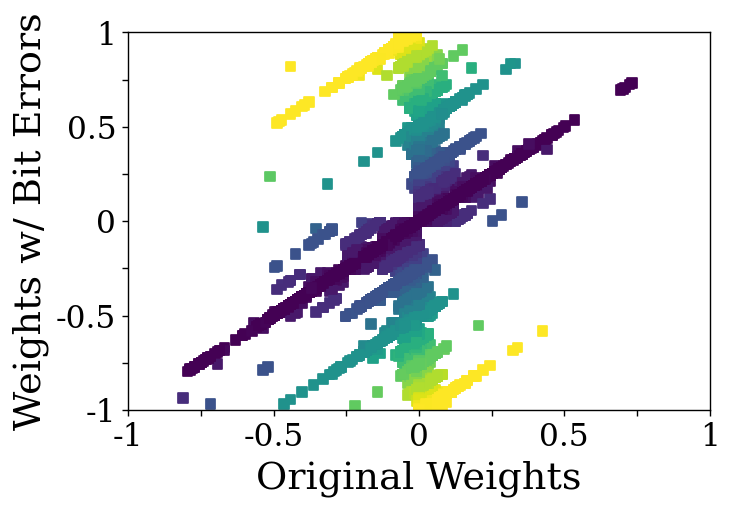
\includegraphics[height=3cm]{c10_errors_q81unfp_nt.png}};
		\node[anchor=north west] at (4,0){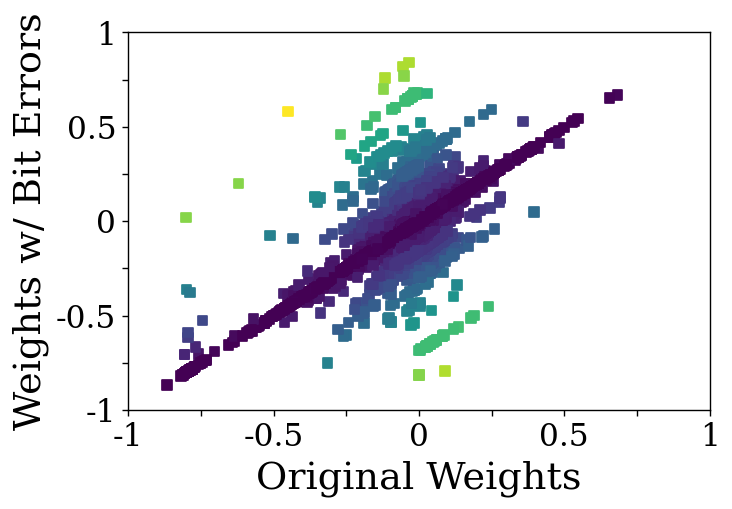
\includegraphics[height=3cm,trim=1cm 0 0 0,clip]{c10_errors_q81aunfp_nt.png}};
		\node[anchor=north west] at (8,0){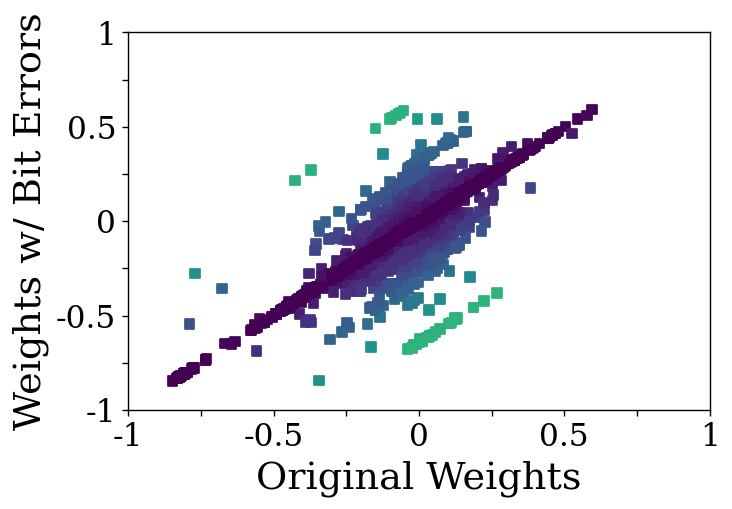
\includegraphics[height=3cm,trim=1cm 0 0 0,clip]{c10_errors_q81auunfp_nt.png}};
		\node[anchor=north west] at (12,0){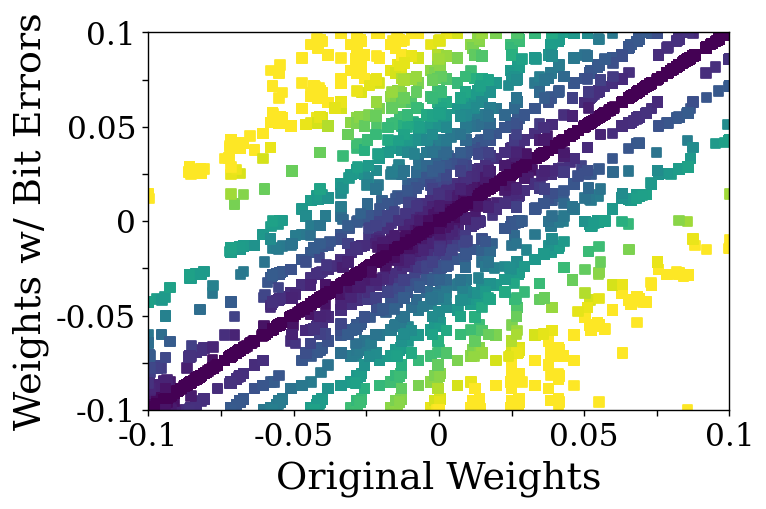
\includegraphics[height=3cm,trim=1cm 0 0 0,clip]{c10_errors_q401auunrfp_nt.png}};
		
		\draw[-,white!50!black] (12.125, 0.25) -- (12.125, -3.25);
		\node[anchor=south,xshift=0.25cm,yshift=-0.25cm] at (2, 0){\textbf{Global}, $\qmax=1$, $m = 8$};
		\node[anchor=south,xshift=0.25cm,yshift=-0.25cm] at (6, 0){\textbf{Per-Layer} (=\Normal)};
		\node[anchor=south,xshift=0.25cm,yshift=-0.25cm] at (10, 0){\textbf{{\color{red}+}Asymmetric}};
		\node[anchor=south,xshift=0.25cm,yshift=-0.25cm] at (14, 0){{\color{red}+}\textbf{\Clipping[$0.1$]}, $m = 4$};
	\end{tikzpicture} 
	\vspace*{-6px}
	\caption{\textbf{Quantization and Random Bit Errors.} Original weights (x-axis) plotted against perturbed weights with bit errors (y-axis), for different %global, per-layer and asymmetric 
	fixed-point quantization schemes with $m = 8$ bit (left) and $p=2.5\%$. We also show the $m = 4$ bit case with \Clipping at $\wmax = 0.1$, \cf \secref{subsec:robustness-clipping}. Color indicates absolute error: from zero {\color{violet}violet} to the maximal possible error {\color{yellow!75!black}yellow} of $1$ (left) and $0.1$ (right). Asymmetric per-layer quantization reduces the impact of bit errors compared to a the symmetric per-layer/global quantization. Clipping reduces absolute error, but the errors \emph{relative} to $\wmax$ increase.}
	\label{fig:quantization}
	\vspace*{-0.2cm}
\end{figure*}